\documentclass[12pt,a4paper]{article}
\usepackage[utf8]{inputenc}
\usepackage[english]{babel}
\usepackage{amsmath}
\usepackage{amssymb}
\usepackage{amsthm}
\usepackage{graphicx}
\usepackage[hidelinks]{hyperref}
\usepackage{bookmark}
\usepackage{listings}
\usepackage{xcolor}
\usepackage{float}
\usepackage{booktabs}
\usepackage{geometry}
\usepackage[ruled,vlined]{algorithm2e}
\usepackage{tikz}
\usetikzlibrary{shapes,mindmap,trees,positioning}
\usepackage{pgfplots}
\pgfplotsset{compat=1.18}
\usepackage{imakeidx}
\makeindex
\usepackage{tcolorbox}
\usepackage{cancel}
\usepackage{pdflscape}
\usepackage{refcount}

% Page margins
\geometry{margin=1in}

% Theorem environments
\theoremstyle{definition}
\newtheorem{definition}{Definition}[section]
\newtheorem{theorem}{Theorem}[section]
\newtheorem{lemma}{Lemma}[section]

% Code listing style
\lstset{
    language=Python,
    basicstyle=\ttfamily\small,
    keywordstyle=\color{blue},
    commentstyle=\color{green!60!black},
    stringstyle=\color{red},
    numbers=left,
    numberstyle=\tiny\color{gray},
    frame=single,
    breaklines=true,
    captionpos=b
}

% Title information
\title{Automatic Reasoning and Planning\\
\large Course Summary - Master's Degree}
\author{Carlos Alberto Botina Carpio\\
Universidad Internacional de la Rioja\\
\href{mailto:carlos.botina621@comunidadunir.net}{carlos.botina621@comunidadunir.net}}
\date{\today}

\begin{document}

\maketitle

\begin{abstract}
This document contains a summary of the Automatic Reasoning and Planning course syllabus for the Master's Degree. It includes a summary of the main topics covered during the sessions, as well as additional explanations and extensions of the concepts and techniques referenced in class. The purpose of this document is to serve as study material and reference for the course contents.

Notice that this document is fully customized to the author's needs, placing greater emphasis on topics that the author struggles with or has not yet mastered, while covering more briefly those topics that are already well understood by the author.

\end{abstract}

\newpage
\tableofcontents
\newpage

% Include section files
\section{Introduction to Decision Making}
\label{sec:decision-making}

Decision making is a complex process that requires evaluating and understanding environmental conditions. In many cases, decisions become so intricate that we need to exhaustively evaluate every possible scenario. This is where mathematics becomes useful in helping us make informed decisions.

When making decisions, the following elements are involved:

\begin{itemize}
    \item \textbf{Future effect}: What is the duration of the decision's impact? (short-term, long-term)
    \item \textbf{Reversibility}: Is it easy to reverse the decision?
    \item \textbf{Impact}: How many areas or domains are affected?
    \item \textbf{Quality}: Ethics, legality, behavioral principles, workplace relationships, etc.
    \item \textbf{Periodicity}: How frequently must this decision be made?
\end{itemize}

\subsection{Decision Classification}
\label{subsec:decision-classification}

Decisions can be classified into two main categories: \textbf{high-level} and \textbf{low-level} decisions. High-level decisions are strategic, have long-term consequences, are difficult to reverse, and affect multiple areas of an organization or system. They are typically exceptional and require careful consideration of various quality factors. In contrast, low-level decisions are operational, have minimal future impact, are easily reversible, and affect fewer areas. They are made frequently and have limited impact on important quality factors.

Table~\ref{tab:decision_classification} summarizes the characteristics that distinguish high-level from low-level decisions based on the elements involved in decision making.

\begin{table}[H]
\centering
\caption{Classification of decisions: High-level vs. Low-level}
\label{tab:decision_classification}
\begin{tabular}{p{4.5cm}p{4.5cm}p{4.5cm}}
\toprule
 & \textbf{High Level} & \textbf{Low Level} \\
\midrule
\textbf{Future Effect} & Affect the future & Don't affect the future \\
\midrule
\textbf{Reversibility} & Difficult reversibility & Reversible \\
\midrule
\textbf{Impact} & Broad impact & Little impact \\
\midrule
\textbf{Quality Factors} & Affect many important & Affect few important \\
\midrule
\textbf{Periodicity} & Exceptional & Frequent \\
\bottomrule
\end{tabular}
\end{table}

Decisions can also be classified as \textbf{programmed} or \textbf{non-programmed}. Programmed decisions have a well-defined step-by-step sequence that is known and can be followed. For example, in case of an emergency, one calls the emergency number. Non-programmed decisions are unique and specific to the situation, with no defined rules or steps to follow.

\subsection{Problem Classification}
\label{subsec:problem-classification}

Problems can be classified as \textbf{structured} or \textbf{non-structured}:

\begin{itemize}
    \item \textbf{Structured problems}: The problem contains all the information needed to solve it. All necessary data, constraints, and conditions are available from the start.
    \begin{itemize}
        \item \textit{Example}: Solving a system of linear equations where all coefficients and constants are given.
    \end{itemize}
    
    \item \textbf{Non-structured problems}: The problem does not contain all the information needed to solve it. To solve it, we need to search for additional information.
    \begin{itemize}
        \item \textit{Example}: Diagnosing a medical condition where symptoms are present but additional tests, patient history, or expert consultation are required to reach a diagnosis.
    \end{itemize}
\end{itemize}


\section{Problem Solving Stages}

\subsection{First Stage: Understand the Problem's Complexity}

There are many techniques to understand a problem's complexity, which can be organized into two main categories:

\begin{itemize}
    \item \textbf{Identify the problem}: Self-questioning about the problem (origin, magnitude, focus, or history), SWOT analysis (Strengths, Weaknesses, Opportunities, Threats), discussion meetings (Scrum), etc.
    
    \item \textbf{Explain the problem}: Go beyond the surface and investigate the underlying causes of the problem. This can be done using various techniques such as ERIM problem classification, the 20 causes technique, the Ishikawa diagram (fishbone diagram), and other root cause analysis methods.

\end{itemize}

We must, therefore, create problem definitions that present characteristics that allow us to work with them efficiently. Some characteristics or assumptions that can be made in simple environments (well-defined problems) are:

\begin{itemize}
    \item \textbf{Discrete}: The world can be conceived in states. In each state there is a finite set of perceptions and actions.
    
    \item \textbf{Accessible}: The agent can access the relevant characteristics of the environment. It can determine the \textbf{current state} of the world and the \textbf{state it would like to reach}.
    
    \item \textbf{Static and deterministic}: There is no temporal pressure nor uncertainty. The world changes only when the agent acts. The result of each action is totally defined and predictable.
\end{itemize}

\subsection{Second Stage: Create a Strategy}

The steps for creating a strategy are:

\begin{enumerate}
    \item \textbf{Define strategies}: Generate potential strategies using techniques such as brainstorming, 4x4x4, etc.
    
    \item \textbf{Choose a strategy}: Select a strategy by evaluating:
    \begin{itemize}
        \item Benefits
        \item Probability of success
        \item Dependencies
        \item Resources needed (time, cost)
    \end{itemize}
    
    \item \textbf{Design the strategy}: Create a roadmap defining which actions will be performed. This involves planning the sequence and details of the actions to be executed.
\end{enumerate}

\subsection{Third Stage: Solve the Problem}

This stage is achieved by implementing the strategy, evaluating the outcome, and if necessary, refining the strategy.



\section{Intelligent Agents}

An \textbf{intelligent agent} is an autonomous entity that perceives its environment through sensors and acts upon that environment through actuators to achieve its goals or objectives. Intelligent agents are characterized by their ability to operate independently, make decisions based on their perceptions, and take actions that affect their environment in pursuit of their goals.

An agent is considered intelligent based on its \textbf{autonomy} and \textbf{rationality}:

\begin{itemize}
    \item \textbf{Autonomy}: The agent operates independently without direct human intervention or control. It has control over its own actions and internal state.
    
    \item \textbf{Rationality}: The agent acts in a way that maximizes its performance measure, given the available information and its knowledge. A rational agent selects actions that are expected to achieve its goals most effectively.
\end{itemize}

\subsection{Phases of Agent Decision Making}

An agent must go through three fundamental phases: \textbf{feel}, \textbf{think}, and \textbf{act}.

\begin{itemize}
    \item \textbf{Feel}: Using perception of the environment through their sensors, the agent extracts and processes information. This phase involves gathering raw data from the environment and converting it into a usable format.
    
    \item \textbf{Think}: The agent reasons and decides through a deliberative process, using the information obtained from the environment and its internal memory. This phase involves analyzing the current situation, considering possible actions, and selecting the best course of action to achieve its goals.
    
    \item \textbf{Act}: Through actuators, the agent produces changes in the environment that will help it achieve its goal. For this, the agent must convert its decisions into information that the actuators can understand and execute.
\end{itemize}

\textit{Example}: Consider a robotic vacuum cleaner agent. In the \textbf{feel} phase, it uses sensors (cameras, bump sensors, dirt detectors) to perceive the room layout, detect obstacles, and identify dirty areas. In the \textbf{think} phase, it processes this information along with its internal map and battery level, deciding which areas to clean next and planning an efficient path. In the \textbf{act} phase, it converts these decisions into motor commands that control its wheels and vacuum mechanism, moving through the room and cleaning the identified areas.


\section{Intelligent Agents Architectures}
\label{sec:agent-architectures}

Agent architectures define the internal structure and organization of an intelligent agent, determining how it processes information, makes decisions, and acts. There are several main types of agent architectures: \textbf{deliberative}, \textbf{reactive}, \textbf{hybrid}, and \textbf{cognitive}.

\subsection{Deliberative Architecture}

A \textbf{deliberative architecture} (also known as a \textit{symbolic} or \textit{thinking} architecture) is characterized by the agent's ability to maintain an internal model of the world and engage in explicit reasoning and planning before taking action. The agent uses symbolic representations of knowledge and performs logical reasoning to determine the best course of action.

\textbf{Key characteristics:}
\begin{itemize}
    \item Maintains an internal model or representation of the world
    \item Uses symbolic knowledge representation
    \item Performs explicit reasoning and planning
    \item Makes decisions based on logical inference
    \item Typically slower to respond but more thoughtful
\end{itemize}


This process involves explicit reasoning and planning, making it a deliberative approach. The agent "thinks before it acts," considering multiple possibilities and their outcomes.

Figure~\ref{fig:deliberative_architecture} illustrates the classic deliberative agent architecture, which follows a Sense-Plan-Act cycle. The architecture consists of three main internal components:

\begin{itemize}
    \item \textbf{Deliberative Planner}: Generates high-level plans based on goals and current state information. It receives failure signals from the monitoring component and creates or refines plans accordingly.
    \item \textbf{Monitoring}: Monitors the execution of the plan, compares the current state with the expected state, and sends failure signals to the planner if deviations occur. It receives plans from the planner and sends specific actions to the execution component.
    \item \textbf{Execution}: Interacts directly with the environment through sensors and actuators. It receives sensor data from the environment, updates the monitoring component with the current state, receives action commands from monitoring, and executes actions in the environment.
\end{itemize}

\begin{figure}[H]
    \centering
    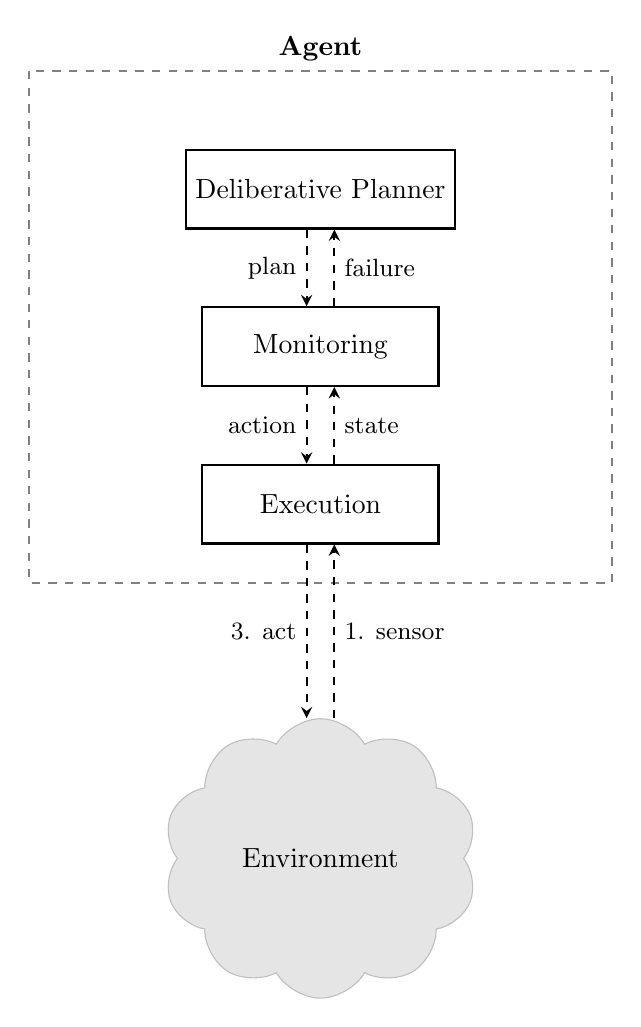
\begin{tikzpicture}[
        box/.style={rectangle, draw=black, thick, minimum width=3cm, minimum height=1cm, align=center},
        env/.style={cloud, draw=gray!50, fill=gray!20, minimum width=4cm, minimum height=2cm, cloud puffs=10, cloud puff arc=120},
        arrow/.style={->, >=stealth, dashed, thick},
        label/.style={font=\small}
    ]
    
    % Agent components (enclosed in dashed box)
    \begin{scope}[local bounding box=agent]
        % Deliberative Planner
        \node[box] (planner) at (0,2) {Deliberative Planner};
        
        % Monitoring
        \node[box] (monitoring) at (0,0) {Monitoring};
        
        % Execution
        \node[box] (execution) at (0,-2) {Execution};
    \end{scope}
    
    % Draw dashed box around agent (ending above environment)
    \draw[dashed, gray, thick] ([shift={(-2cm,1cm)}]agent.north west) rectangle ([shift={(2cm,-0.5cm)}]agent.south east);
    \node[above] at ([shift={(0,1cm)}]agent.north) {\textbf{Agent}};
    
    % Environment (outside agent boundaries)
    \node[env] (env) at (0,-6.5) {Environment};
    
    % Arrows
    % Environment to Execution (sensor) - UP arrow, goes on the right
    \draw[arrow] ([xshift=5pt]env.north) -- node[right, label] {1. sensor} ([xshift=5pt]execution.south);
    
    % Execution to Environment (act) - DOWN arrow, goes on the left
    \draw[arrow] ([xshift=-5pt]execution.south) -- node[left, label] {3. act} ([xshift=-5pt]env.north);
    
    % Execution to Monitoring (state)
    \draw[arrow] ([xshift=5pt]execution.north) -- node[right, label] {state} ([xshift=5pt]monitoring.south);
    
    % Monitoring to Execution (action)
    \draw[arrow] ([xshift=-5pt]monitoring.south) -- node[left, label] {action} ([xshift=-5pt]execution.north);
    
    % Monitoring to Deliberative Planner (failure)
    \draw[arrow] ([xshift=5pt]monitoring.north) -- node[right, label] {failure} ([xshift=5pt]planner.south);
    
    % Deliberative Planner to Monitoring (plan)
    \draw[arrow] ([xshift=-5pt]planner.south) -- node[left, label] {plan} ([xshift=-5pt]monitoring.north);
    
    \end{tikzpicture}
    \caption{Classic deliberative agent architecture (Sense-Plan-Act cycle)}
    \label{fig:deliberative_architecture}
    \end{figure}
    

The flow operates as a continuous cycle:
\begin{enumerate}
    \item The agent \textbf{senses} the environment through sensors (1. sensor), providing raw data to the Execution component.
    \item Execution updates Monitoring with the current \textbf{state}.
    \item Monitoring compares the state with the \textbf{plan} received from the Deliberative Planner and determines the next \textbf{action} for Execution. If the plan is not progressing as expected, Monitoring sends a \textbf{failure} signal to the Deliberative Planner.
    \item The Deliberative Planner receives failure signals and generates or refines a \textbf{plan}, which is sent to Monitoring.
    \item Execution \textbf{acts} (3. act) upon the environment based on the action received from Monitoring.
\end{enumerate}

This cycle represents how a deliberative agent continuously perceives, plans, and acts to achieve its goals, with a mechanism for detecting and responding to plan failures.

\subsubsection{Examples of Deliberative Architectures}

\begin{itemize}
    \item \textbf{Planning agents}: These agents use automated planning algorithms to generate sequences of actions that achieve specific goals. They maintain a symbolic representation of the world state and use search algorithms to find optimal or near-optimal plans. Planning agents are commonly used in robotics, autonomous systems, and game AI where complex sequences of actions need to be coordinated.

    \item \textbf{Belief Desire \& Intention (BDI)}: This architecture models agents based on three mental attitudes: \textbf{Beliefs} (what the agent knows about the world), \textbf{Desires} (the agent's goals or objectives), and \textbf{Intentions} (the commitments to specific plans of action). BDI agents reason about their beliefs, select desires to pursue, and commit to intentions (plans) to achieve those desires. This architecture is particularly useful for modeling complex, goal-oriented behavior in multi-agent systems and autonomous agents.
    
\end{itemize}


\subsection{Reactive Architecture}

A \textbf{reactive architecture} (also known as a \textit{behavior-based} architecture) is characterized by the agent's direct mapping from perceptions to actions without maintaining an internal world model or engaging in complex reasoning. The agent responds quickly to environmental stimuli through simple stimulus-response rules.

\textbf{Key characteristics:}
\begin{itemize}
    \item No internal world model or symbolic representation
    \item Direct mapping from sensors to actuators
    \item Simple stimulus-response rules or behaviors
    \item Fast response time
    \item Emergent behavior from simple rules
\end{itemize}

\textit{Example}: Consider a simple obstacle-avoidance robot with a reactive architecture. The robot has sensors on its front and sides, and it follows these simple rules:
\begin{itemize}
    \item If the front sensor detects an obstacle, turn right
    \item If the right sensor detects an obstacle, turn left
    \item If no obstacles are detected, move forward
    \item If both sensors detect obstacles, move backward
\end{itemize}

The robot doesn't maintain a map of its environment or plan a path. It simply reacts to what it perceives at each moment. This makes it very fast and efficient for simple tasks, though it may not find the optimal path. The robot's navigation behavior emerges from these simple reactive rules.

Figure~\ref{fig:reactive_planner_architecture} illustrates a reactive agent architecture that incorporates a \textbf{Reactive Planner} component:

\begin{itemize}
    \item \textbf{Reactive Planner}: Positioned at the top, this component generates reactive action sequences in direct response to the current state. Unlike deliberative planners, it does not maintain a complex world model but instead quickly generates actions based on immediate perceptions. It receives failure signals from Monitoring and sends actions back to Monitoring.
    \item \textbf{Monitoring}: Positioned in the middle, it monitors the execution of actions and the current state. It receives state information from Execution, sends failure signals to the Reactive Planner when deviations occur, receives actions from the Reactive Planner, and sends action commands to Execution. It also receives external plans.
    \item \textbf{Execution}: Located at the bottom, it interacts directly with the environment through sensors and actuators. It receives sensor data from the environment, updates Monitoring with the current state, receives action commands from Monitoring, and executes actions in the environment.
\end{itemize}


\begin{figure}[H]
    \centering
    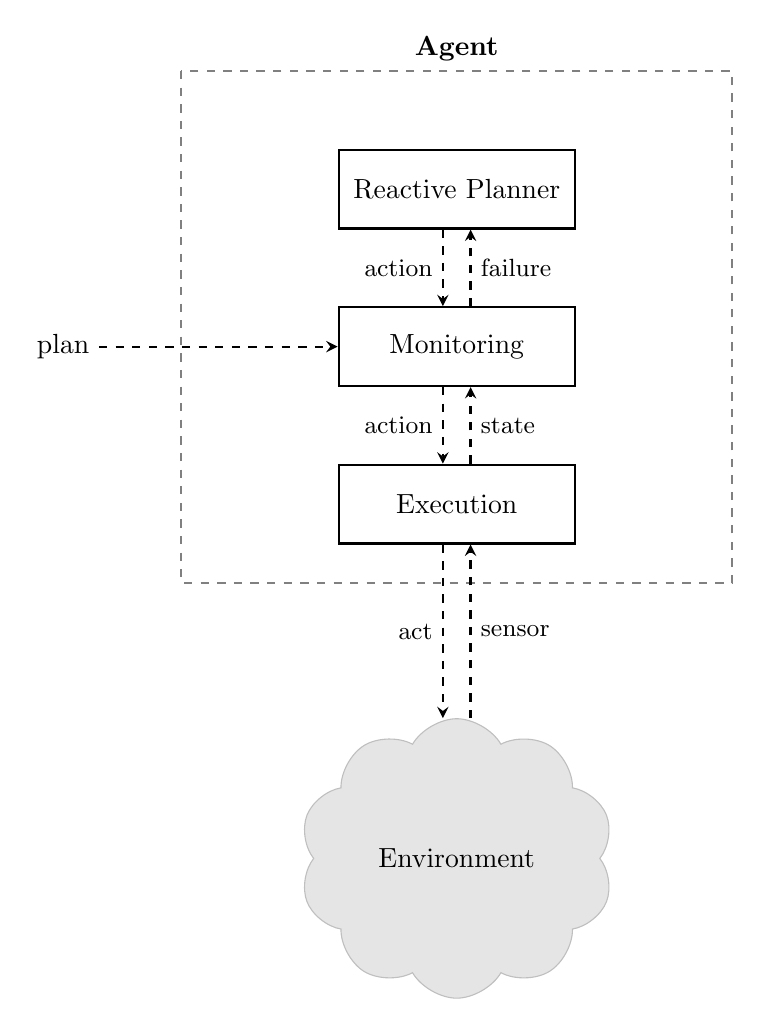
\begin{tikzpicture}[
        box/.style={rectangle, draw=black, thick, minimum width=3cm, minimum height=1cm, align=center},
        env/.style={cloud, draw=gray!50, fill=gray!20, minimum width=4cm, minimum height=2cm, cloud puffs=10, cloud puff arc=120},
        arrow/.style={->, >=stealth, dashed, thick},
        label/.style={font=\small}
    ]
    
    % Agent components (enclosed in dashed box)
    \begin{scope}[local bounding box=agent]
        % Reactive Planner (top) - centered
        \node[box] (reactive_planner) at (0,2) {Reactive Planner};
        
        % Monitoring (middle) - centered
        \node[box] (monitoring) at (0,0) {Monitoring};
        
        % Execution (bottom) - centered
        \node[box] (execution) at (0,-2) {Execution};
    \end{scope}
    
    % Draw dashed box around agent (ending above environment)
    \draw[dashed, gray, thick] ([shift={(-2cm,1cm)}]agent.north west) rectangle ([shift={(2cm,-0.5cm)}]agent.south east);
    \node[above] at ([shift={(0,1cm)}]agent.north) {\textbf{Agent}};
    
    % Plan source (outside agent boundaries, to the left of monitoring)
    \node (plan_source) at (-5,0) {plan};
    
    % Environment (outside agent boundaries)
    \node[env] (env) at (0,-6.5) {Environment};
    
    % Arrows
    % Plan to Monitoring
    \draw[arrow] (plan_source.east) -- node[above, label] {} (monitoring.west);
    
    % Environment to Execution (sensor) - UP arrow, goes on the right
    \draw[arrow] ([xshift=5pt]env.north) -- node[right, label] {sensor} ([xshift=5pt]execution.south);
    
    % Execution to Environment (act) - DOWN arrow, goes on the left
    \draw[arrow] ([xshift=-5pt]execution.south) -- node[left, label] {act} ([xshift=-5pt]env.north);
    
    % Execution to Monitoring (state)
    \draw[arrow] ([xshift=5pt]execution.north) -- node[right, label] {state} ([xshift=5pt]monitoring.south);
    
    % Monitoring to Reactive Planner (failure)
    \draw[arrow] ([xshift=5pt]monitoring.north) -- node[right, label] {failure} ([xshift=5pt]reactive_planner.south);
    
    % Reactive Planner to Monitoring (action)
    \draw[arrow] ([xshift=-5pt]reactive_planner.south) -- node[left, label] {action} ([xshift=-5pt]monitoring.north);
    
    % Monitoring to Execution (action)
    \draw[arrow] ([xshift=-5pt]monitoring.south) -- node[left, label] {action} ([xshift=-5pt]execution.north);
    
    \end{tikzpicture}
    \caption{Reactive agent architecture with Reactive Planner}
    \label{fig:reactive_planner_architecture}
    \end{figure}



The flow operates as follows:
\begin{enumerate}
    \item An external \textbf{plan} is provided to the Monitoring component (this could come from a higher-level planner or user input).
    \item The Environment sends \textbf{sensor} data to the Execution component, providing raw information about the current state of the environment.
    \item Execution processes the sensor data and updates Monitoring with the current \textbf{state}.
    \item Monitoring evaluates the state against the plan. If there is a deviation or problem, it sends a \textbf{failure} signal to the Reactive Planner.
    \item The Reactive Planner receives the failure signal and immediately generates a reactive \textbf{action} response, which it sends back to Monitoring.
    \item Monitoring receives the action from the Reactive Planner and forwards the \textbf{action} command to Execution.
    \item Execution \textbf{acts} upon the environment based on the action received from Monitoring.
\end{enumerate}

This architecture emphasizes fast, reactive responses to environmental changes while still allowing for external plan guidance. The Reactive Planner provides quick adaptation without the overhead of maintaining complex internal models. The bidirectional flow between Monitoring and the Reactive Planner enables rapid failure detection and action generation.

\subsubsection{Examples of Reactive Architectures}

\begin{itemize}
    \item \textbf{Subsumption architecture}: A layered architecture where behaviors are organized in levels of increasing complexity. Lower-level behaviors (like obstacle avoidance) can subsume or override higher-level behaviors (like exploration) when triggered by environmental conditions. Each layer operates independently and reactively, with no central control or world model.
    
    \item \textbf{Agent network architecture from Pattie Maes}: A distributed reactive architecture where multiple simple agents (or behaviors) are connected in a network. Each agent has local rules and can activate or inhibit other agents. The overall behavior emerges from the interactions between these agents, without centralized planning.
    
    \item \textbf{Reactive execution model}: Is domain independent and operates with structures precalculated at runtime.
\end{itemize}

\subsection{Hybrid Architecture}
\label{subsec:hybrid}

A \textbf{hybrid architecture} combines elements of both deliberative and reactive architectures. It typically has multiple layers: a reactive layer for fast, immediate responses to critical situations, and a deliberative layer for complex planning and reasoning. This architecture attempts to get the best of both worlds: the speed of reactive systems and the intelligence of deliberative systems.

\textbf{Key characteristics:}
\begin{itemize}
    \item Combines reactive and deliberative components
    \item Multiple layers of control (reactive at the bottom, deliberative at the top)
    \item Fast response for urgent situations (reactive layer)
    \item Complex reasoning and planning for strategic decisions (deliberative layer)
    \item Coordination between layers
\end{itemize}

\textit{Example}: Consider an autonomous vehicle with a hybrid architecture. The vehicle has two main layers:

\begin{itemize}
    \item \textbf{Reactive layer}: Handles immediate, critical situations. For example:
    \begin{itemize}
        \item If a pedestrian suddenly appears in front, immediately apply brakes (no time for planning)
        \item If another vehicle swerves into the lane, quickly adjust steering
    \end{itemize}
    
    \item \textbf{Deliberative layer}: Handles strategic planning and navigation. For example:
    \begin{itemize}
        \item Plans the route from origin to destination
        \item Analyzes traffic conditions and selects the best path
        \item Decides when to change lanes based on traffic patterns
        \item Maintains a map and tracks the vehicle's position
    \end{itemize}
\end{itemize}

The reactive layer ensures safety by responding instantly to immediate threats, while the deliberative layer handles the overall navigation strategy. The layers work together: the deliberative layer sets the general plan, and the reactive layer handles unexpected situations that require immediate action.

\subsubsection{Examples of Hybrid Architectures}

\begin{itemize}
    \item \textbf{Procedural Reasoning System (PRS)}: A BDI (Belief-Desire-Intention) architecture that combines deliberative reasoning with reactive capabilities. The agent maintains \textbf{Beliefs} (facts about the world expressed in first-order logic), \textbf{Desires} (system behaviors or goals), and \textbf{Intentions} (the current set of active plans). PRS includes a library of partially specified plans called Knowledge Areas (KAs), each with an activation condition. KAs can be activated by goals or by data, and can be reactive, allowing PRS to respond quickly to environmental changes while also reasoning about which plans to execute.
    
    \item \textbf{COSY (Cooperative System)}: A BDI architecture that combines elements from both PRS and IRMA architectures. It has five main components: \textbf{Sensors} (receive perceptual inputs), \textbf{Actuators} (perform actions), \textbf{Communications} (send messages), \textbf{Cognition} (mediates between intentions and knowledge to choose actions), and \textbf{Intention} (contains long-term goals and control elements). COSY combines deliberative reasoning with reactive communication and action capabilities, making it suitable for interactive and collaborative environments.
\end{itemize}


\subsection{Cognitive Architecture}

A \textbf{cognitive architecture} is a computational framework that models the structure and processes of human cognition. It provides a unified theory of how the mind works, including perception, memory, reasoning, learning, and decision-making. Cognitive architectures can be defined as a hypothesis about the fixed structures that provide a mind, whether in natural or artificial systems, and how they work together—along with the knowledge and skills incorporated within the architecture—to produce intelligent behavior in a diversity of complex environments. Cognitive architectures aim to create artificial agents that can exhibit human-like intelligence and behavior.

\textbf{Key characteristics:}
\begin{itemize}
    \item Models human cognitive processes and structures
    \item Provides unified framework for multiple cognitive functions
    \item Includes memory systems (short-term and long-term)
    \item Supports learning and adaptation
    \item Integrates perception, reasoning, and action
    \item Based on cognitive science and psychology principles
\end{itemize}

\subsubsection{Examples of Cognitive Architectures}

\begin{itemize}
    \item \textbf{ACT-R}: A cognitive architecture developed primarily by John Robert Anderson at Carnegie Mellon University. The most important assumption of ACT-R is that human knowledge can be divided into two irreducible types of representations:
    \begin{itemize}
        \item \textbf{Declarative knowledge}: Represented as \textbf{chunks} (vector representations of individual properties, each accessible from a labeled slot)
        \item \textbf{Procedural knowledge}: Represented as production rules
    \end{itemize}
    Chunks are maintained and accessed through \textbf{buffers}, which are the front-end of \textbf{modules} (specialized and largely independent brain structures). ACT-R has two main types of modules:
    \begin{itemize}
        \item \textbf{Perceptual-motor module}: Handles interaction with the environment, managing the flow of perception and action necessary to connect the agent with the world
        \item \textbf{Memory module}: Divided into:
        \begin{itemize}
            \item \textbf{Long-term memory} (production memory): Contains production rules
            \item \textbf{Short-term memory} (working memory or declarative memory): Contains current facts about the world
        \end{itemize}
    \end{itemize}
     
    \item \textbf{SOAR}: A cognitive architecture created at Carnegie Mellon University by Laird, Newell, and Rosenbloom (1987). The ultimate goal of SOAR is to provide a foundation for a system capable of general intelligent behavior, supporting the full range of cognitive tasks, problem-solving methods, and knowledge representations. SOAR is both a theory of cognition and a computational implementation of that theory.
    
    The design of SOAR is based on the hypothesis that all goal-oriented deliberate behavior can be understood as the selection and application of \textbf{operators} to a \textbf{state}:
    \begin{itemize}
        \item \textbf{State}: A representation of the current problem situation
        \item \textbf{Operator}: Transforms a state (performs changes in the representation)
        \item \textbf{Goal}: A desired result for the problem
    \end{itemize}
    SOAR runs continuously, attempting to apply the current operator and select the next operator (a state can have only one operator at a time) until the goal is achieved.
    
    SOAR has separate memories with different representation modes:
    \begin{itemize}
        \item \textbf{Short-term memory}: Stores sensor data, intermediate inferences about current data, currently active goals, and active operators (actions and plans)
        \item \textbf{Long-term memory} (production memory): Maintains knowledge for responding to situations through procedures. It stores problem-solving knowledge, inference rules, and knowledge for selecting and applying operators in specific states
    \end{itemize}
\end{itemize}


\subsection{Other Architectures}

\begin{itemize}
    \item Three layer architecture
    \item Multilayer architecture
    \item Three tower architecture
\end{itemize}





% Summary
\clearpage
\section{Summary}

\begin{figure}[p]
\centering
\resizebox{\textwidth}{!}{
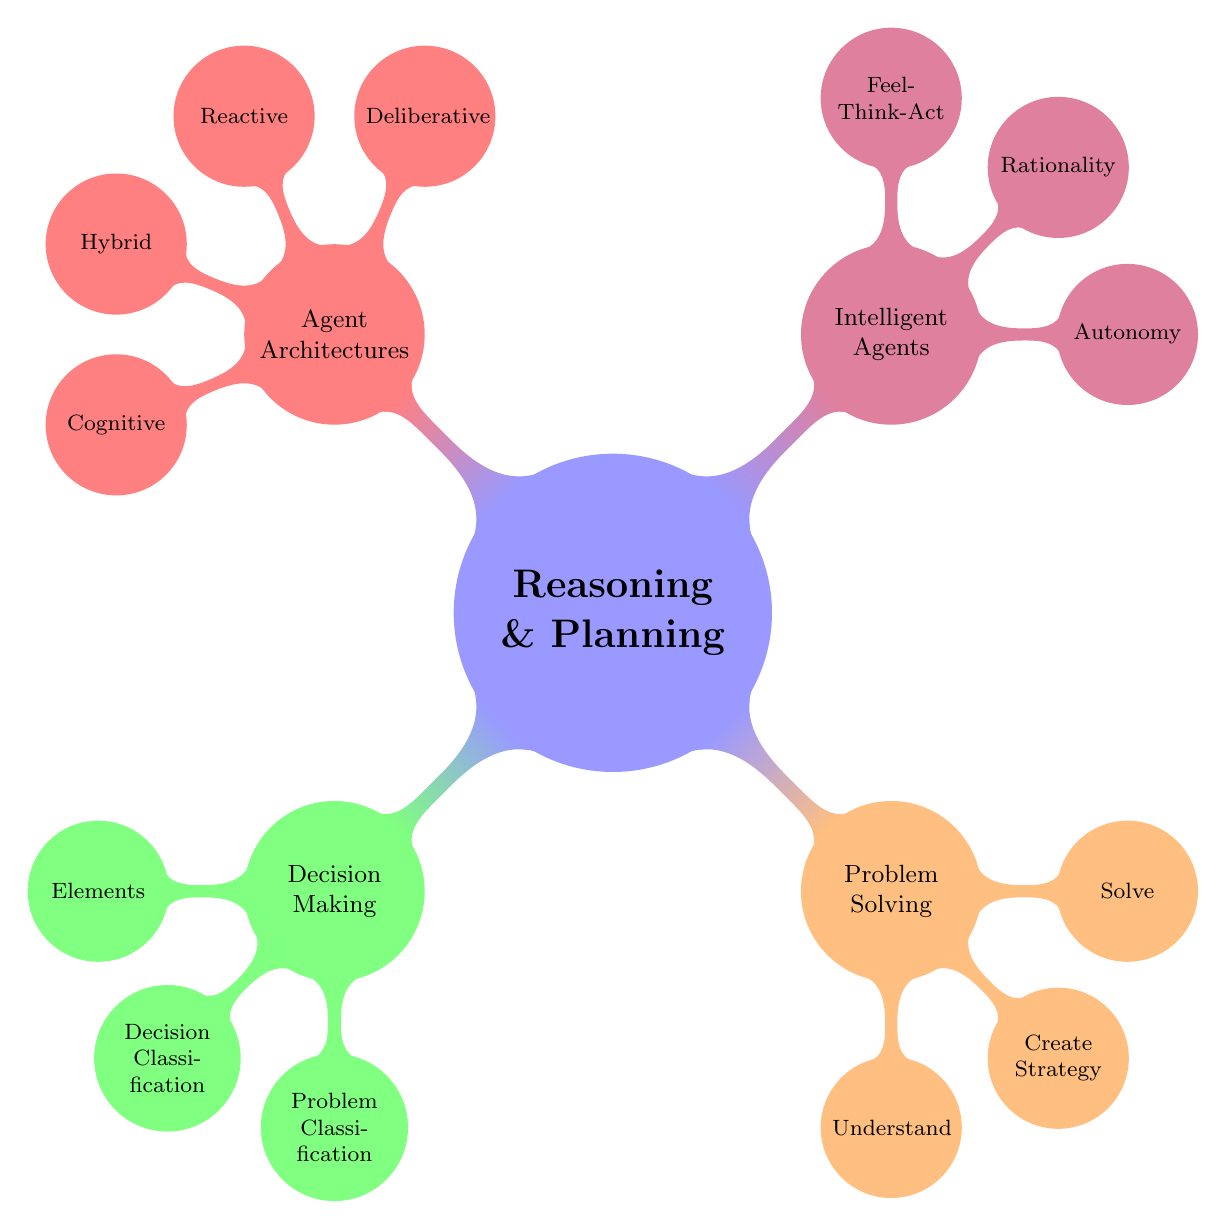
\begin{tikzpicture}[
    mindmap,
    grow cyclic,
    every node/.style=concept,
    concept color=blue!40,
    level 1/.append style={level distance=5cm,sibling angle=90},
    level 2/.append style={level distance=3cm,sibling angle=45},
]

% Central concept
\node[concept,font=\Large\bfseries] {Reasoning \& Planning}
    % Decision Making branch
    child[concept color=green!50] {
        node[concept] {Decision Making}
        child {node[concept] {Elements}}
        child {node[concept] {Decision Classification}}
        child {node[concept] {Problem Classification}}
    }
    % Problem Solving branch
    child[concept color=orange!50] {
        node[concept] {Problem Solving}
        child {node[concept] {Understand}}
        child {node[concept] {Create Strategy}}
        child {node[concept] {Solve}}
    }
    % Intelligent Agents branch
    child[concept color=purple!50] {
        node[concept] {Intelligent Agents}
        child {node[concept] {Autonomy}}
        child {node[concept] {Rationality}}
        child {node[concept] {Feel-Think-Act}}
    }
    % Agent Architectures branch
    child[concept color=red!50] {
        node[concept] {Agent Architectures}
        child {node[concept] {Deliberative}}
        child {node[concept] {Reactive}}
        child {node[concept] {Hybrid}}
        child {node[concept] {Cognitive}}
    };

\end{tikzpicture}
}
\caption{High-level overview of the Reasoning and Planning course structure}
\end{figure}

\subsection*{Key Concepts Summary}

\begin{itemize}
    \item \textbf{Decision Making}: Understanding decision complexity, elements involved (future effect, reversibility, impact, quality, periodicity), and classification of decisions and problems.
    
    \item \textbf{Problem Solving Stages}: Three-stage approach: (1) Understand the problem's complexity through identification and explanation techniques, (2) Create a strategy by defining, choosing, and designing, (3) Solve by implementing, evaluating, and refining.
    
    \item \textbf{Intelligent Agents}: Autonomous and rational entities that perceive their environment through sensors (Feel), reason and decide using deliberative processes (Think), and execute actions through actuators (Act).
    
    \item \textbf{Agent Architectures}:
    \begin{itemize}
        \item \textit{Deliberative}: Maintain internal world models and perform explicit reasoning (e.g., Planning agents, BDI)
        \item \textit{Reactive}: Direct stimulus-response without world models (e.g., Subsumption, Agent networks)
        \item \textit{Hybrid}: Combine deliberative and reactive approaches (e.g., PRS, COSY)
        \item \textit{Cognitive}: Model human cognitive processes with memory systems (e.g., ACT-R, SOAR)
    \end{itemize}
\end{itemize}



\end{document}
